\chapter{Introduction}

\section{Background and Motivation}
[Your background and motivation section goes here. This should introduce the general area of your research and explain why your work is important. Typically 2-3 paragraphs.]

Lorem ipsum dolor sit amet, consectetur adipiscing elit. Sed do eiusmod tempor incididunt ut labore et dolore magna aliqua. Ut enim ad minim veniam, quis nostrud exercitation ullamco laboris nisi ut aliquip ex ea commodo consequat.

\section{Research Objectives}
The main objectives of this research are:
\begin{enumerate}
\item [First objective: Describe what you aim to achieve]
\item [Second objective: Another key goal of your research]
\item [Third objective: Additional research aim if applicable]
\end{enumerate}

\section{Research Questions}
This study addresses the following research questions:
\begin{enumerate}
\item [Research Question 1: What specific question are you investigating?]
\item [Research Question 2: Another question your research addresses]
\end{enumerate}

\section{Methodology Overview}
[Brief overview of your research methodology. This should be 1-2 paragraphs describing your general approach.]

\section{Example Figures}
This section demonstrates how to include figures in your thesis. Figure \ref{fig:research_overview} shows a general overview of the research process, while Figure \ref{fig:methodology} illustrates the methodology framework.

\begin{figure}[h!tbp]
\centering
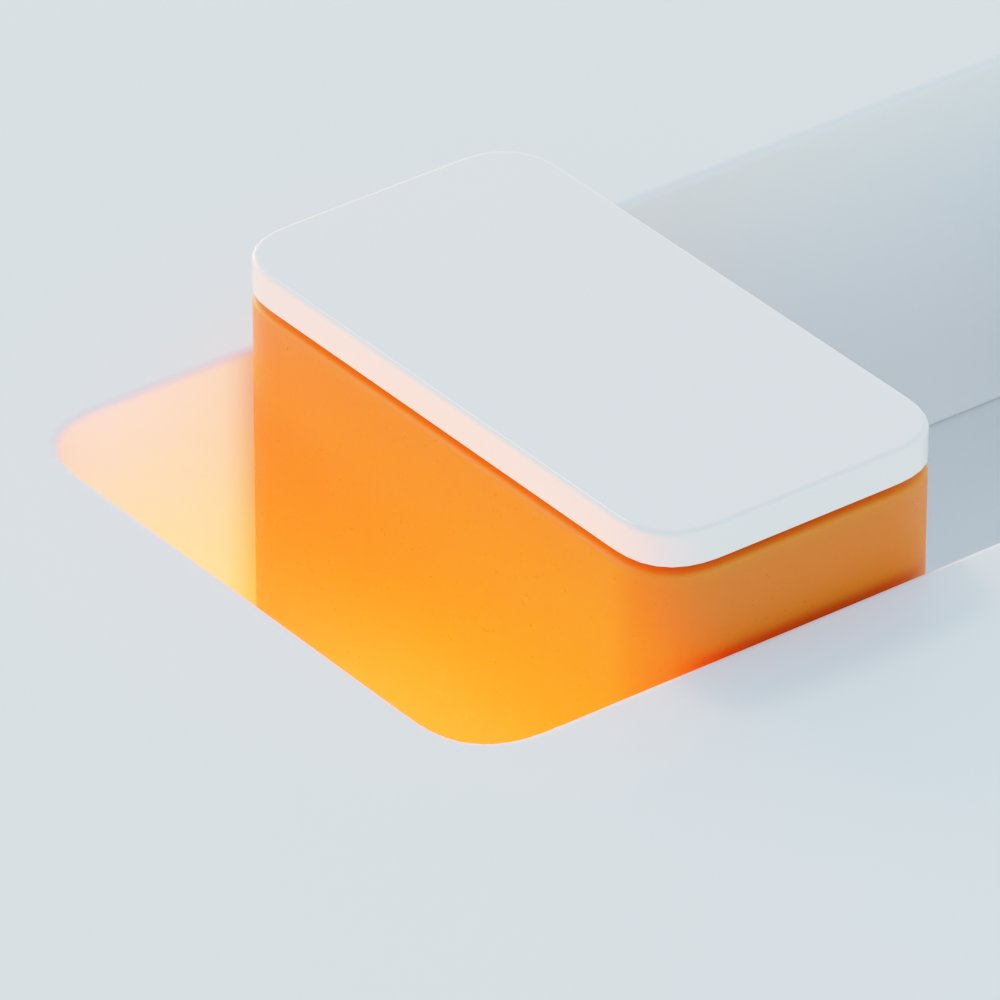
\includegraphics[width=0.7\textwidth]{chapters/1/figures/fig_1.png}
\caption{Research overview and key components. This figure demonstrates how to include and reference figures in your thesis.}
\label{fig:research_overview}
\end{figure}

\begin{figure}[h!tbp]
\centering
\includegraphics[width=0.7\textwidth]{chapters/1/figures/fig_2.png}
\caption{Methodology framework and approach. This shows the systematic approach to conducting research.}
\label{fig:methodology}
\end{figure}

\section{Thesis Structure}
This thesis is organized as follows:
\begin{itemize}
\item Chapter 1: Introduction - Provides background, objectives, and methodology
\item Chapter 2: Literature Review - Reviews relevant previous work and establishes context
\item [Additional chapters as needed for your specific research]
\end{itemize}

\section{Expected Contributions}
[Describe the expected contributions of your research to the field. What new knowledge or insights will your work provide?]
